\documentclass[conference]{IEEEtran}
\IEEEoverridecommandlockouts


%%
%% Submission ID.
%% Use this when submitting an article to a sponsored event. You'll
%% receive a unique submission ID from the organizers
%% of the event, and this ID should be used as the parameter to this command.
%%\acmSubmissionID{123-A56-BU3}
\usepackage{cite}
\usepackage{amsmath,amssymb,amsfonts}
\usepackage{algorithmic}
\usepackage{graphicx}
\usepackage{textcomp}
\usepackage{xcolor}
\usepackage{listings}
\usepackage{caption}
\usepackage{subcaption}
\usepackage{array}

\definecolor{backcolor}{rgb}{0.95,0.95,0.92}

\lstdefinestyle{mystyle}{
  basicstyle=\ttfamily\footnotesize,
  keywordstyle=\color{blue},
  stringstyle=\color{red},
  commentstyle=\color{green},
  breakatwhitespace=true,
  breaklines=true,
  keepspaces=true,
  showspaces=false,
  showstringspaces=false,
  showtabs=false,
  tabsize=4,
  captionpos=b,
  numbers=left,
  numberstyle=\tiny\color{gray},
  backgroundcolor=\color{backcolor},
}
\lstset{style=mystyle}
\usepackage{graphicx}
\usepackage{caption}

\def\BibTeX{{\rm B\kern-.05em{\sc i\kern-.025em b}\kern-.08em
    T\kern-.1667em\lower.7ex\hbox{E}\kern-.125emX}}

\begin{document}

\title{Bridging the Gap Between Visual and Analytical Machine Learning
  Testing}

\author{\IEEEauthorblockN{1\textsuperscript{st} Given Name Surname}
\IEEEauthorblockA{\textit{dept. name of organization (of Aff.)} \\
\textit{name of organization (of Aff.)}\\
City, Country \\
email address or ORCID}
\and
\IEEEauthorblockN{2\textsuperscript{nd} Given Name Surname}
\IEEEauthorblockA{\textit{dept. name of organization (of Aff.)} \\
\textit{name of organization (of Aff.)}\\
City, Country \\
email address or ORCID}
\and
\IEEEauthorblockN{3\textsuperscript{rd} Given Name Surname}
\IEEEauthorblockA{\textit{dept. name of organization (of Aff.)} \\
\textit{name of organization (of Aff.)}\\
City, Country \\
email address or ORCID}
}

\maketitle

\begin{abstract}
Testing ML systems is a highly interactive process which demands a
human-in-the-loop approach. In addition to writing tests for the code
base, practitioners are required to analyse and interpret several
visualisations using their domain expertise to validate if an ML
system satisfies the required set of functional and non-functional
properties. Visualisations are frequently used to qualitatively assess
various parts of an ML pipeline. However, implicit knowledge gained
from visualisations must be translated to explicit analytical tests
that fail when there is change in any component of the ML pipeline. We
conduct an empirical analysis of Jupyter notebooks to catalogue the
state-of-the-art mappings between ML visualisations and assertions. We
mine Github to collect Jupyter Notebooks that contain assertions
written in Python. We develop a novel methodology to identify 1764
notebooks which contain an assertion below a visualisation. We
manually analyse the 1.7K notebooks and identify 551 notebooks where
at least one pair of visualisation and assertion are semantically
related to one another. We further read and understand 90 notebooks in
depth to identify 26 qualitative and their corresponding quantitative
testing patterns. We showcase five such patterns in this paper and
plan to make the entire catalogue publicly available in the near
future.
\end{abstract}

\begin{IEEEkeywords}
  ML Testing, Visualisations, ???
\end{IEEEkeywords}

\section{Introduction}\label{sec:intro}

Recent years show a shift from chasing high correctness of ML models
to ensuring that they are safe for application in safety-critical
domains such as healthcare, finance and autonomous driving. With the
advent of Large Language Models, the power of AI to directly influence
the daily lives of humans is growing at a radical pace. As reports of
``hallucinated'' facts, racist predicts and autonomous car crashes
steadily increase, ensuring that ML systems function as they were
intended to, takes precedence.

Visualisations are used throughout the ML development lifecycle to
test various properties of the ML system. In the early stages of the
ML development lifecycle, visualisations are extensively used for make
sense of the data and verify its statistical properties. During the
model development phase, visualisations are used to summarise metrics
and contrast different learning algorithms and iteratively fine-tune
ML models. Once the model is deployed in production, visualisations
are used to continually monitor their performance and trigger a new
training cycle once their performance drops below a certain threshold.

Building ML systems is highly iterative and experimental. Information
gained from ML visualisations is used to make design and
implementation decisions for the following steps of the ML
pipeline. For instance, we may visualise the distribution of our
training data and find that it is normally distributed. Based on this
information, we may opt for a Linear Regression model which assumes
normality in the underlying data. However, such expectations regarding
the data may be violated once the ML system is deployed in production,
where the data constantly changes as a reflect of the real
world. Implicit expectations obtained from visualisations must
therefore be translated to analytical tests that fail once our
expectations regarding the ML system are no longer satisfied.

In contrast to prior work done in ML testing, we approach this
pressing topic from a novel direction. We conduct an empirical
analysis of computational notebooks obtained from Github, to
understand the process of testing ML systems in practice. In
particular, we focus on the combination of a qualitative form of
testing (using visualisations) and a qualitative form of testing
(using analytical assertions). The research questions along with the
contributions of this paper are as follows.

\begin{description}
\item[RQ1.] How frequently do ML practitioners formulate analytical
  tests from the visualisations they create to test ML systems?

We mine 54K Jupyter notebooks from Github that contain an assertion
    written in Python. We develop an automated technique to identify
    1764 notebooks with an assertion below a visualisation. We
    manually analyse the 1.7K notebooks and identify 551 notebooks
    that contain at least one pair of visualisation and assertion that
    are semantically related to each other.

\item[RQ2.] What are the types of visualisation and assertion pairs
  typically used by ML practitioners when testing ML systems?

From the 551 notebooks, we further perform an in-depth analysis of 90
    notebooks. We identify 26 unique visualisation and assertion
    pairs. We discuss five such pairs in this paper and plan to
    release the full catalogue publicly in the near future.
\end{description}

% TODO what are the primary findings of this paper...

The paper is organised as follows. Section~\ref{sec:prelim} summarises
the related literature and technical information relevant to this
study. The methodology for the empirical study is explained in
Section~\ref{sec:method} and the results of the study are presented in
Section~\ref{sec:result}. The paper concludes with a discussion on the
implications of our results (Section~\ref{sec:discuss}), threats to
validity (Section~\ref{sec:threats}) and future work
(Section~\ref{sec:conclude}).

\section{Preliminaries}\label{sec:prelim}

% TODO how is our work different from prior work?

This section summarises the body of prior scientific work that has
been done in ML Testing, computational notebooks and visual
analytics. The section concludes with an overview of technical
knowledge required for this paper.

\subsection{ML Testing}\label{sec:ml-testing}

Testing ML enabled software systems poses more challenges compared to
their traditional counter part. While traditional software systems
mature through change in their codebase, ML enabled systems experience
change in the training data and the machine learning model in addition
to the codebase\cite{CITEME}. With ML being adopted into
safety-critical domains that can affect human lives, ensuring that ML
systems are correct, robust to data perturbations and not biased by
race, colour or gender is of paramount importance. Existing scientific
literature on ML testing broadly focuses on two aspects. First, on
functional properties such as correctness and robustness of the model
towards unseen data. And second, on non-functional properties such as
fairness, interpretability and privacy.

To test the correctness of ML models, several improvements over
existing test adequacy metrics have been proposed. Tools such as
\textit{DeepExplore} and \textit{DeepGauge} propose new test adequacy
metrics such as neuron coverage adapted for ML enabled software
systems~\cite{pei2017deepexplore, ma2018deepgauge,
gerasimou2020importance}. Formal verification methods have also been
proposed that try to provide formal guarantee of robustness against
adversarial examples. Such methods however are only feasible for
statistical ML models and become computationally expensive for more
complex models such as deep neural networks~\cite{zhu2021deepmemory,
baluta2021scalable}. Several works have been conducted on generating
and detecting adversarial inputs for ML models. Data augmentation
techniques based on fuzzing, search based software testing and
mutation testing have been proposed to generate adversarial examples
that can be used during model training to improve its
robustness~\cite{braiek2019deepevolution, gao2020fuzz, wang2021robot,
zhang2020white}. It is however not possible to include all variations
of adversarial examples into the training data. Thus, methods have
been proposed to detect adversarial inputs during
runtime~\cite{xiao2021self, wang2020dissector, wang2019adversarial,
berend2020cats}.

% TODO summarise literature on fairness testing
Bulk of the contributions on testing non-functional properties of ML
systems, focuses on fairness.

\subsection{Computational Notebooks and Software
  Engineering}\label{sec:notebooks}

Computational notebooks have been ubiquitously adopted by the machine
learning community for developing ML enabled systems. Although
originally intended to promote reproducible software, computational
notebooks are far from being reproducible due to lack of software
engineering best practices such as separation of concern, testing and
versioning~\cite{pimentel2019large}.

\cite{psallidas2019data} provide an overview of the evolving landscape
of computational notebooks by analysing six million Python notebooks,
two million enterprise data science pipelines, and source code and
metadata from over 900 releases of 12 important data science
libraries. Their findings can be used by system builders for improving
data science tools and also by data science practitioners to
understand the current trends and what technologies they should focus
on. \cite{pimentel2019large} mined 1.4 million notebooks from Github
to conduct an empirical study on the good and bad coding practices in
computational notebooks. Based on their analysis, the authors propose
guidelines on improving reproducibility of computational notebooks. To
enable future research on computational notebooks,
\cite{quaranta2021kgtorrent} mine Kaggle~\footnote{https://kaggle.com}
and present \textit{KGTorrent}, a public dataset consisting of
approximately 2.5 million Jupyter notebooks written in Python. The
dataset also contains a relational database dump of metadata regarding
publicly available notebooks on Kaggle.

Studies with human subjects have been conducted to gain a deeper
understanding of the challenges faced by ML practitioners when
developing ML models inside notebooks. The results indicate that ML
practitioners work in a highly iterative fashion, often experimenting
with multiple strategies to analyse the data or produce meaningful
visualisations~\cite{kandel2012enterprise, kery2018story,
liu2019understanding, chattopadhyay2020wrong}. Studies have also been
conducted to understand how practitioners generate, evaluate and
manage alternative hypothesis, visual designs, methods, tools,
algorithms and data sources to arrive at the final
implementation~\cite{liu2019understanding,kandel2012enterprise}. The
findings from these studies can be used as guidelines for improving
existing notebook technologies or designing new ones.

To manage and prune the multiple versions of code that accumulate over
time when developing in notebooks, \cite{head2019managing} propose
a code gathering tool that allows practitioners to review and only
keep the relevant version of code. Other tools such as
\textit{WrangleDoc} and \textit{VizSmith} have also been proposed to
aid ML practitioners when working within computational
notebooks~\cite{yang2021subtle, bavishi2021vizsmith}.

\subsection{Visualisations and Machine Learning}\label{sec:visualisations}

As ML augment software systems in safety-critical domains, emphasis
has been put into explainability of ML models. ML models and the
underlying data is complex and multi-dimensional. To combat the
``curse of dimensionality'', visual analytics has been widely adopted
by the ML community to understand the data and the internal workings
of ML models.

Prior studies have been conducted to understand how visual analytics
techniques are currently being used in ML. \cite{yuan2021survey}
conduct a systematic review of 259 papers and propose a taxonomy of
visual analytics techniques for ML. \cite{hohman2019visual} conduct
a survey of visual analytics techniques for Deep Learning Models. The
findings of the study indicate that visual analytics has been widely
adopted in ML for model explanation, interpretation, debugging and
improvement.

Several tools have been proposed by the visual analytics research
community to aid practitioners in understanding how their ML models
operate. \cite{wexler2020if} propose \textit{What-If}, a visual
analytics tool to explore alternative hypotheses, generate
counterfactual reasoning, investigate decision boundaries of the model
and how change in data affects the model predictions. To reduce the
cognitive load of ML practitioners during model building phase,
\cite{amershi2015modeltracker} propose \textit{ModelTracker}. Given
a trained model and a sample dataset, ModelTracker presents all the
information in traditional summary statistics along with the
performance of the model.

\textit{ESCAPE}, \textit{GAM Coach}, \textit{Angler} and
\textit{Drava} are a few other tools that have been proposed to handle
specialised use-cases such as identifying systemmatic errors in ML
models, generating counterfactual explanations for Generalised
Additive Models, prioritising machine translation model improvements
and relating human concepts with semantic dimensions extracted by ML
models during disentangled representation learning\cite{ahn2023escape,
wang2023gam, robertson2023angler, wang2023drava}.

\subsection{Internal Structure of Jupyter Notebooks}\label{sec:nbformat}

\begin{minipage}{0.45\textwidth}
  \begin{lstlisting}
{
  "metadata": {
    "kernel_info": {...},
    "language_info": {...},
  },
  "nbformat": 4,
  "nbformat_minor": 0,
  "cells": [ # dictionary of all cells in notebook ]
}
  \end{lstlisting}
  \captionof{lstlisting}{Top-level JSON format of Jupyter notebooks.
    See Listing~\ref{lst:cell-md},~\ref{lst:cell-code}
    and~\ref{lst:cell-output} for internal structure of various
    cells.}\label{lst:nbformat}
\end{minipage}
\hfill
\begin{minipage}{0.45\textwidth}
  \begin{lstlisting}
{
  "cell_type": "markdown",
  "metadata": {},
  "source": [
    "# Hello world example\n",
    "The following cell contains python code for greeting people!\n"
  ]
}
  \end{lstlisting}
  \captionof{lstlisting}{JSON structure of markdown cells.}
  \label{lst:cell-md}
\end{minipage}
\begin{minipage}{0.45\textwidth}
  \begin{lstlisting}
{
  "cell_type": "code",
  "metadata": {},
  "source": [
    "def greet(name):\n",
    "    print(f'Hello, {name}!')\n"
  ]
}
  \end{lstlisting}
  \captionof{lstlisting}{JSON structure of code cells.}
  \label{lst:cell-code}
\end{minipage}
\hfill
\begin{minipage}{0.45\textwidth}
  \begin{lstlisting}
{
  "cell_type": "code",
  "metadata": {},
  "source": [...],
  "outputs": [
    {
      "output_type": "display_data",
      "data": {
        "image/png": "<base64-encoded-png-data>"
      }
    }
  ]
}
  \end{lstlisting}
  \captionof{lstlisting}{JSON structure of code cells with an image output.}
  \label{lst:cell-output}
\end{minipage}

The data comprised within Jupyter Notebooks is stored in the JSON
format, and thus can be parsed
programmatically. Listing~\ref{lst:nbformat} shows the top-level json
structure of Jupyter Notebooks, adopted from the official nbformat
website.~\footnote{https://nbformat.readthedocs.io/en/latest/index.html}. For
simplicity, we only show the parts that are relevant for this study
and hide the irrelevant parts using ellipsis.

Notebooks contain four top level keys namely \texttt{metadata},
\texttt{nbformat}, \texttt{nbformat\_minor} and \texttt{cells}. The
\texttt{matadata} key consists of additional information regarding the
notebook such as the kernel and programming
language. \texttt{nbformat} and \texttt{nbformat\_minor} contain the
version of nbformat used in the notebook. The \texttt{cells} key
consists of a list of all cells within the notebook.

Listings~\ref{lst:cell-md},~\ref{lst:cell-code} and
~\ref{lst:cell-output} present three examples of cells. Each cell is
represented as a dictionary with the \texttt{cell\_type},
\texttt{metadata} and \texttt{source} keys. Cells can be of three
types: ``markdown'', ``code'' or ``raw''. The contents of each cell
can be found within the \texttt{source} key, as a list of strings.

Outputs generated by a code cell are stored as a list within the
\texttt{outputs} key as seen in Listing~\ref{lst:cell-output}. Static
visualisations are stored as base64 encoded png images under the
\texttt{"image/png"} key, which is nested within the \texttt{data} key
inside \texttt{outputs}.

\subsection{Post-Condition Checks}\label{sec:post-cond}

\begin{table*}
\centering
\caption{Frequent examples of post-condition checks observed in this study.}
  \begin{tabular}{m{0.3\textwidth} m{0.4\textwidth} m{0.3\textwidth}}
\hline
\emph{\textbf{Visualisation}}&
\emph{\textbf{Post-condition check}}&
\emph{\textbf{Rationale}}\\
\hline
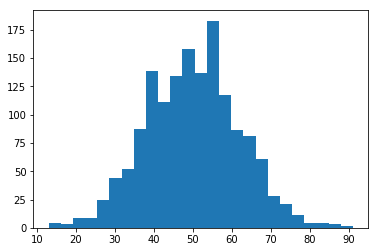
\includegraphics[width=\linewidth]{post-cond-01.png}&
\begin{lstlisting}[language=Python]
assert f1.gca().has_data()
\end{lstlisting}&
The assertion checks if the output of the visualisation code cell contains an image.\\
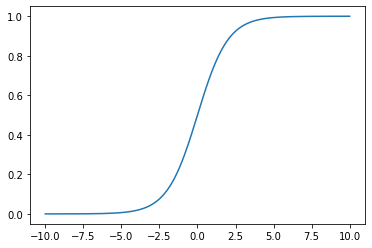
\includegraphics[width=\linewidth]{post-cond-02.png}&
\begin{lstlisting}[language=Python]
assert_almost_equal(sigmoid(-50), 0, delta=1e-10)
assert_almost_equal(sigmoid(0), 0.5, delta=1e-10)
assert_almost_equal(sigmoid(50), 1, delta=1e-10)
\end{lstlisting}&
The assertions are spot-checking the sigmoid activation function.\\
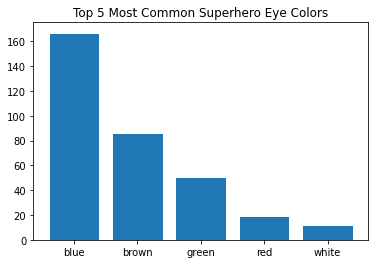
\includegraphics[width=\linewidth]{post-cond-03.png}&
\begin{lstlisting}[language=Python]
# The axis should contain 5 bars
assert len(ax.containers[0]) == 5

# One of the x tick labels should be "blue"
tick_text = [tick.get_text() for tick in ax.get_xticklabels()]
assert "blue" in tick_text
\end{lstlisting}&
The asserts are validating the correctness of the visualisation itself.\\
\hline
\end{tabular}
\label{tab:post-cond}
\end{table*}

We found several instances of visualisation and assertion pairs which
were realated to one another. However the assertions did not test
a property of the ML system that was derived from the
visualisation. Instead, the assertions were used to test the
correctness of the code that produced the visualisation. Such
assertions (and the corresponding visualisations) were excluded from
this study. Table~\ref{tab:post-cond}provides examples of
post-condition checks which were frequently observed in this study.

\section{Methodology}\label{sec:method}
Figure~\ref{fig:method} presents an overview of all relevant steps
used in this study. The empirical analysis comprises of three distinct
phases namely: \textit{the data collection phase},
\textit{identification of related visualisation and assertion pairs}
and finally a \textit{complete analysis of the notebooks} to identify
the final set of 26 visualisation and assertion pairs.

The yellow boxes in the data collection phase represent filters that
were applied to the initial corpus of 54K notebooks, to obtain the
final sample size of 1.7K notebooks used in the empirical study. The
red boxes represent the exclusion criteria used during phase two to
remove notebooks note relevant for this study. Finally, the green
boxes in phase 3 represent the manual analysis conducted to identify
the final 26 visualisation and assertion pairs.

Boxes appearning next to one-another imply that they were applied
using an "OR" operator. While boxes appearning below one-another imply
an "AND" operator. Text in double quotes represent the string pattern
used in the search query. Each phase of the methodology is explained
in more detail below.

\begin{figure*}
  \centering
  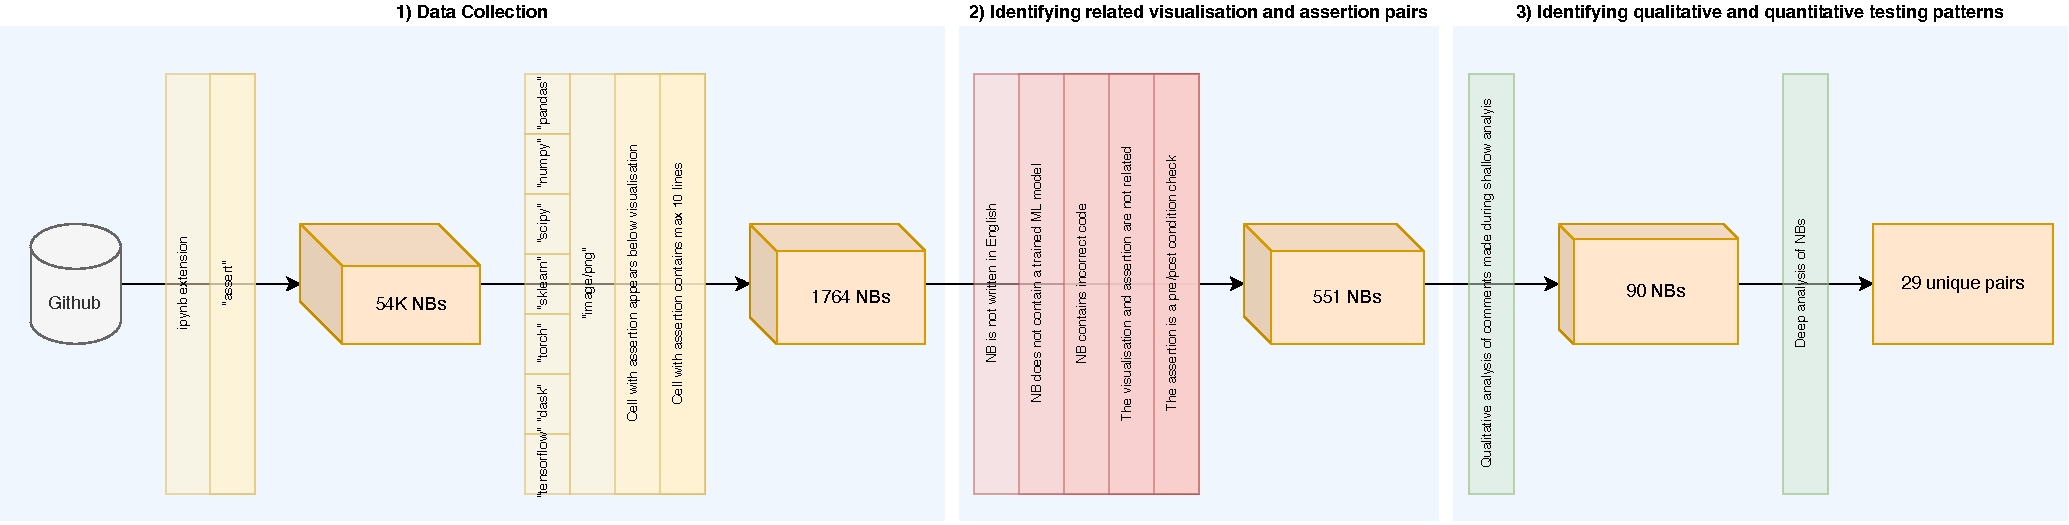
\includegraphics[width=\textwidth]{method.pdf}
  \caption{Methodology used to collect and analyse Jupyter notebooks
    in this study.}
  \label{fig:method}
\end{figure*}

\subsection{Data Collection}\label{sec:data-collect}

We mined public repositories from Github to collect Jupyter notebooks
that contain the keyword ``assert'' in them. We intentionally keep the
search criteria on Github broad by only checking for the appropriate
filetype and the presence of the ``assert'' keyword. This is because,
the ``assert'' keyword is used in python to define
tests. Additionally, popular python libraries which provide a testing
interface (such as nose, unittest and numpy), contain the same keyword
in their API. Our search criteria captures a large initial sample of
$54,070$ notebooks with a variety of testing statements. Our approach
also prevents the need to craft a custom search query based on an
exhaustive list of keywords that appear in all python testing
libraries.

We use the Github advanced search syntax~\footnote{REFME} to isolate
Jupyter Notebook. This translates to the following Github search
query: \texttt{filename:"Jupyter Notebooks"}. Additionally, we include
the ``assert'' keyword in the search query with an \texttt{AND}
operator. The final search query is as follows:
\texttt{filename:"Jupyter Notebooks" AND "assert"}.

The above search query results in approximately 54K notebooks. To
further reduce the sample size, we exclude notebooks that do not use
popular ML libraries. We perform a string search to identify notebooks
that import at least one of the ML libraries. The string patterns are
derived from the python module name used in the import statements. The
regex search query is as follows:
\texttt{tensorflow|dask|torch|sklearn|scipy|numpy|pandas}.

We programmatically parse the JSON structure of the notebooks and
represent each notebook as a pandas dataframe for further analysis. We
map each cell as a row in the dataframe. For each cell, we store the
\texttt{cell\_type}, the \texttt{source} of the cell and the base64
encoded PNG string, into the corresponding columns of the
dataframe. We exclude notebooks that do not contain any visualisations
by checking if the image column of the dataframe is empty. The
internal structure of Jupyter notebooks is presented in
Section~\ref{sec:nbformat}.

\begin{figure*}
  \centering
  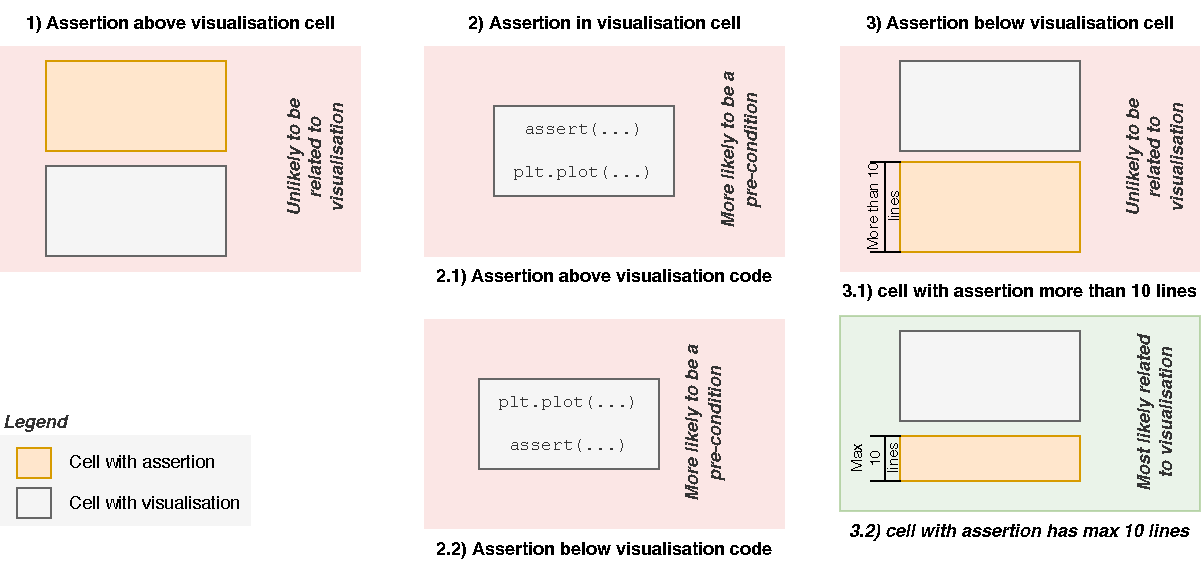
\includegraphics[width=\textwidth]{nb-structure.pdf}
  \caption{Arrangement of code cells containing assertion and
    visualisation.}
  \label{fig:cell-arrangement}
\end{figure*}

For RQ1, we are interested in finding empirical evidence of
visualisations and corresponding assertions used in the wild. To
answer this question, we further reduce our notebook sample size by
assuming a specific order in which the visualisation and assertion
code cells appear in the notebooks. Figure~\ref{fig:cell-arrangement}
presents a visual representation of various arrangements of code cells
that may occur in notebooks. Note that the visual representation omits
markdown cells since we only consider the order of code cells in our
analysis. In the actual notebook however, one or more markdown cells
may be present between the visualisation and assertion cells.

We conduct the manual analysis presented in
Section~\ref{sec:identify-related-pairs} for a small random sample of
notebooks containing each cell arrangement. We observed the
signal-to-noise ratio for each cell arrangement and picked the
arrangement with the highest signal-to-noise
ratio. Table~\ref{tab:cell-arrangement} presents the cell arrangement
in ascending order of signal-to-noise ratio with a summary of our
observations.

Assertions defined in a cell above the visualisation cell, were
typically not related to each other. Often, a markdown cell present
between the assertion and visualisation code cells, would mark the
begining of a new section in the notebook. In other cases, the
assertions were typically checks to ensure that the visualisation code
would not encounter any errors. This observation also holds for
Arrangement 2.1, where the assertion is defined above the
visualisation code, in the same cell. Common examples of such checks
include checking the shape of features that are used in the
visualisation. Or checking that the length of the ``x''and ``y``
features are the same to ensure a continuous line in the plot.

The signal-to-noise ratio was observed to improve in the sample of
notebooks where the assertions were defined below the visualisation
code. The visualisation and assertions pairs observed in Arrangment
2.2 and 3.1 were often related to each other, but were post-condition
checks. Section~\ref{sec:post-cond} provides more details on
post-condition checks and our rationale for excluding them from this
study.

We observed the best results in notebooks where the assertion cell was
not longer than 10 lines and was defined below the visualisation cell
(Arrangement 3.2). We observed that most notebook authors followed the
convention of writing their motivation for the visualisation in
a markdown cell, before writing the code for the visualisation. The
visualisations were often followed by another markdown cell to record
the author's observations. And finally, the observations were
translated to a analytical test using \texttt{``assert''} or other
testing methods from external libraries. The restriction on the number
of lines in the assertion cell was introduced to exclude instances
where the assertion cell contained a new class definition or several
helper functions that were not related to the visualisation above.

\begin{table}
  \centering
  \caption{Observations from random samples of notebooks with various
  cell arrangement.}
  \begin{tabular}{l p{0.2\textwidth} p{0.2\textwidth}}
    \hline
    \emph{\textbf{ID}}&
    \emph{\textbf{Cell arrangement}} &
    \emph{\textbf{Observations}}\\
    \hline
    1 &
    Assertion cell above visualisation cell &
    Least likely to be related to the visualisation below.\\
    \hline
    \multicolumn{3}{l}{\textbf{Assertion and visualisation in the same code cell}}\\
    \hline
    2.1 &
    Assertion above visualisation code &
    More likely to be a pre-condition check.\\
    2.2 &
    Assertion below visualisation code &
    More likely to be a post-condition check.\\
    \hline
    \multicolumn{3}{l}{\textbf{Assertion cell below visualisation cell}}\\
    \hline
    3.1 &
    Assertion cell more than 10 lines &
    Better signal-to-noise ratio compared to Arrangement 2.1. However, More likely to be post-condition check or unrelated to the visualisation above.\\
    3.2 &
    Assertion cell has max 10 lines &
    Most likely to be related to the visualisation above.\\
    \hline
  \end{tabular}
  \label{tab:cell-arrangement}
\end{table}

\subsection{Identifying Related Visualisation and Assertion Pairs}\label{sec:identify-related-pairs}

The initial sample size of 54K notebooks from Github, was reduced to
the final sample size of 1.7K after applying the filters presented in
Section~\ref{sec:data-collect}. We analysed all 1.7K notebooks
manually to further identify 551 notebooks that contained at least one
pair of visualisation and assertions that were related to each
other. Table~\ref{tab:exclusion-criteria} presents the exclusion
criteria used in this phase of the analysis, along with the number of
notebooks that were excluded based on each criteria.

We manually analysed the source code of the visualisation and
assertion. And excluded visualisation and assertion pairs that were
not related to each other. We encountered several instances where the
tracing was not straightforward due to poor coding practices. In such
cases, we used one-shot prompt engineering~\cite{CITME} with the
ChatGPT 4.0 model to determine if the visualisation and assertion were
related to each other.

We excluded notebooks that did not train an ML model. We found several
notebooks authored on topics such as linear algebra, optimisation and
loss functions. Although these topics are related to ML, the
visualisation and assertion pairs found in these notebooks could not
be readily applied to a typically ML development workflow. Analysing
such notebooks also required a working knowledge of all mathematical
concepts related to ML. This was deemed beyond the scope of software
engineering research.

Finally, we excluded notebooks that were not authored in English or
contained faulty code that did not produce
a visualisation. Table~\ref{tab:exclusion-criteria} lists all
exclusion criteria used along with the number of notebooks that were
excluded from this study.

\begin{table}
  \centering
  \caption{Exclusion criteria used to identify related visualisation and assertion pairs.}
  \begin{tabular}{l p{0.2\textwidth} r}
    \hline
    \textbf{ID} &
    \textbf{Exclusion Criteria} &
    \textbf{Num. excluded NBs}\\
    \hline
    \textbf{EC1} &
    The visualisation and assertion are not related &
    440\\
    \textbf{EC2} &
    Notebook does not contain a trained ML model &
    383\\
    \textbf{EC3} &
    The assertion is a post-condition check &
    200\\
    \textbf{EC4} &
    Notebook not written in English &
    159\\
    \textbf{EC5} &
    Notebook contains incorrect code &
    31\\
    \hline
    \multicolumn{2}{c}{\emph{\textbf{Total number of NBs excluded:}}} &
    1.213\\
    \hline
  \end{tabular}
  \label{tab:exclusion-criteria}
\end{table}

\subsection{Deeper Analysis of Notebooks}\label{sec:deep-dive}

We qualitatively assess the comments made for all notebooks during the
analysis conducted in phase two of the study, as described in
Section~\ref{sec:identify-related-pairs}. 

We perform an in-depth analysis of 90 short-listed notebooks to
identify unique ML testing tasks. The in-depth analysis was conducted
by reading and understanding the entire contents of the notebooks in
a top-down order. During the analysis, we note several data points
such as the primary objective of the notebook, the type of ML problem,
the type of ML model and the type of data. We manually read and
comprehend each code cell in the notebooks. When present, we also read
the markdown cells above and below code cells to gain further context
from the notebook author. For instance, we find that markdown cells
above a visualisation cell typically motivates the need for the
visualisation. A markdown cell directly below a visualisation often
records the observations made by the notebook author from the
visualisation.

\section{Results}\label{sec:result}

% TODO move the stuff for RQ1 from methodology here!

% NOTE the 5 pairs is to illustrate the 26 total pairs/approach we found for testing ML systems

% NOTE visual+analytical test is a new "strategy" for testing AI

This study identified 26 patterns of testing using visualisation and
assertion. This section highlights five interesting patterns in more
detail. We plan to release the entire catalogue of patterns publicly
in the near future.


\subsection{Decision boundary}\label{sec:svm}

% NOTE something about how the visualisation helps with interpretability of how the model is classifying the data?

% NOTE the author is using the visualisation to iteratively check/test how different kernels perform on the data; can also use it for hyper-parameter tuning?

% NOTE: visualisation can provide qualitative assessment of under/overfitting

% NOTE: better assertion: perhaps on the support vectors?

% NOTE assertion created was a single metric (performance): we need tools/guidelines to help practitioners capture what they see in visualisations; community failing to help practitioners what they are visualising

% NOTE assertion is not capturing the whole thing, only assert == we lose a lot of info, we need both

\begin{figure}
  \subcaptionbox{Visualisation of the decision boundary of a SVM with a linear kernel.\label{fig:svm-linear}}{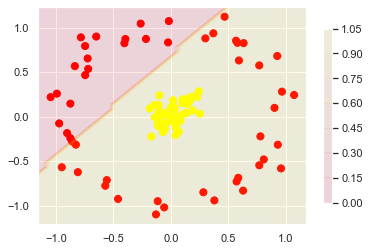
\includegraphics[width=0.45\linewidth]{../catalogue/select-04-linear.png}}
  \hfill
  \subcaptionbox{Visualisation of the decision boundary of a SVM with a RBF kernel.\label{fig:svm-rbf}}{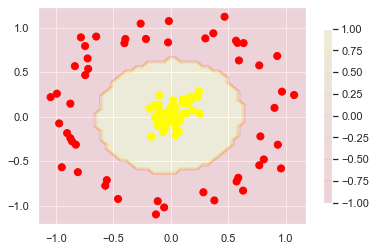
\includegraphics[width=0.45\linewidth]{../catalogue/select-04-rbf.png}}
  \caption{Visualisation of the decision boundary of a SVM trained using different kernels.}
  \label{fig:svm}
\end{figure}
\begin{lstlisting}[language=Python]
assert accuracy_score(y_test, pred) > 0.95
\end{lstlisting}
\captionof{lstlisting}{Assertion on the accuracy of the ML model.}\label{lst:svm}

Figures~\ref{fig:svm} presents visualisations obtained from a notebook that performs binary classification using Support Vector Machines (SVM). The model is trained on the \texttt{make\_circles}~\footnote{REFME} dataset obtained from scikit-learn~\footnote{REFME}. The visualisations show the two classes present in the training set, and the decision boundary of the model when trained first using a linear kernel (Figure~\ref{fig:svm-linear}) and later with a RBF kernel (Figure~\ref{fig:svm-rbf}).

% NOTE maybe we need to ellaborate; the linear kernel was above the rbf; based on observations from the linear kernel, the author decides to try the rbf kernel; then after experimenting with hyper-parameters the author puts an assertion that captures the model's performance at that specific point in time.

The visualisations presented in Figure~\ref{fig:svm} contain several useful information that can be used to test and debug ML models. Humans are tuned to recognise visual patterns~\cite{CITEME}. Visualisations in Figure~\ref{fig:svm}, allows ML practitioners to quickly identify mis-classified examples. Additionally, observing the complexity of the decision boundary is a quick way to determine if the model is under or overfitting the data. For instance, in Figure~\ref{fig:svm-linear} we observe that the model is underfitting since a linear kernel too simply for the underlying data. The visualisation also allows ML practitioners to compare different ML models or variants of the same ML model to iteratively find a model that best fits the underlying training data. In this case for instance, the author of the notebook First trained the SVM with a linear kernel. And upon realising that the data is not linearly separable, chose the RBF kernel.

Listing~\ref{lst:svm} shows the corresponding assertion that was defined below the visualisations. The assertion checks if the model accuracy is above a threshold specified by the author of the notebook. The assertion is derived from the observations made from the visualisation in Figure~\ref{fig:svm-rbf}. The visulisation shows that the model is able to classify the data well which is why the notebook author sets the threshold for the accuracy in the assertion to a high value.

The assertion however, is only able to capture the information pertaining to the performance of the model. While the rest of the information that is gained from the qualitative assessment using visualisation is lost.

\subsection{Input Image, \texttt{predict\_proba}}

\begin{figure}
  \subcaptionbox{Random input image of a football from the test set.\label{fig:football}}{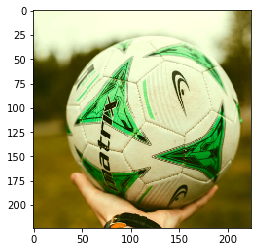
\includegraphics[width=0.45\linewidth]{../catalogue/select-35a.png}}
  \hfill
  \subcaptionbox{Random input image of tennis balls from the test set.\label{fig:tennisball}}{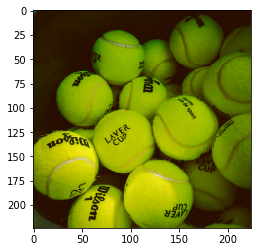
\includegraphics[width=0.45\linewidth]{../catalogue/select-35b.png}}
  \caption{Visualisation of random input images for a pre-trained image classifier.}
  \label{fig:balls}
\end{figure}

\begin{minipage}{0.45\textwidth}
  \begin{lstlisting}[language=Python]
np.testing.assert_almost_equal(pred_proba, 2.0355723e-05, decimal=3)
  \end{lstlisting}
  \captionof{lstlisting}{Assertion below Figure~\ref{fig:football}. It checks if the probability estimate of the model is close to the specified value. The input image is of a football. Since the model is trained to detect tennis balls, the specified value is very small.}
  \label{lst:football}
\end{minipage}
\hfill
\begin{minipage}{0.45\textwidth}
  \begin{lstlisting}[language=Python]
np.testing.assert_almost_equal(pred_proba, 0.9988895, decimal=3)
  \end{lstlisting}
  \captionof{lstlisting}{Assertion below Figure~\ref{fig:tennisball}. Compared to Listing~\ref{lst:football}, the specified value is much higher, since the input image contains tennis balls.}
  \label{lst:tennisball}
\end{minipage}

Figure~\ref{fig:balls} presents visualisations obtained from a notebook that uses a pre-trained image classifier from the GluonCV library~\footnote{https://cv.gluon.ai}, to identify images that contain tennis balls. The visualisations are of two random input images, one from each class in the dataset. Listing~\ref{lst:football} presents the assertion related to Figure~\ref{fig:football}. The assertion checks if the probability estimate of the model for the given input image, is close to the specified value with a precision of up to three decimal places. Since the model is trained to detect tennis ball, and the input image contains a footbal, the specified probability estimate is very low. In contrast, Listing~\ref{lst:tennisball} specifies a much higher probability estimate since the input image contains tennis balls.

The above visualisation and assertion pair can be used to spot-check a few edge-cases or adversarial examples which the model may find difficult to classify. It is unclear however, how the specified thresholds were obtained since the authors do not provide additional explanation in the notebook. The threshold may have been derived based on the domain expertise of the ML practitioner. Another alternative could be to define them during the Requirements Engineering phase, by discussing with all involved stakeholders\cite{CITEME}.

In contrast to the visualisation and assertion pair in Section~\ref{sec:svm}, the assertion here is able to capture the author's motivation for visualising the input image along with the information obtained from it. Regardless, the notebook author still visualises the input image. This is a recurring phenomenon that we observe in other visualisation and assertion pairs in our catalogue. We discuss this phenomenon further in Section~\ref{sec:visual}.

\subsection{Normality}\label{sec:normal}

\begin{minipage}{0.45\textwidth}
  \begin{lstlisting}[language=Python]
for feature in range(data_transformed.shape[1]):
  assert kstest(data_transformed[:, feature], 'norm').statistic < 1e-2
  \end{lstlisting}
  \captionof{lstlisting}{Assertion to check that each feature in a dataset is normal. The distribution of each feature is compared to that of a normal distribution using the Kolmogorov-Smirnov test for goodness of fit from the scipy library.}
  \label{lst:kstest}
\end{minipage}
\hfill
\begin{minipage}{0.45\textwidth}
  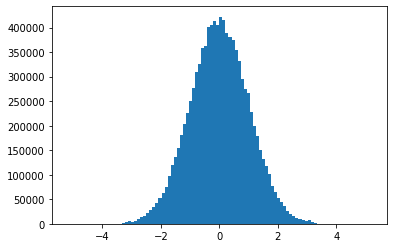
\includegraphics[width=\linewidth]{../catalogue/select-152a.png}
  \captionof{figure}{Visualisation of the distribution of a feature from the dataset.}
  \label{fig:kstest}
\end{minipage}

% NOTE assertion and viz are perfect fit; 

% NOTE despite the analytical test, practitioners need to visualise this, we need visual confirmation; we cannot get rid of visualisations. we need both!

The visualisation in Figure~\ref{fig:kstest} is obtained from a notebook that trains a Generative Adversarial Network (GAN) to generate data which simulates a neutrino particle detector. The notebook author transforms the training data by normalising it using the \texttt{QuantileTransform} from scikit-learn~\footnote{REFME}. After performing the transformation, the author performs a visual check by plotting the distribution of a feature from the dataset as shown in Figure~\ref{fig:kstest}. The visualisation shows a bell-shaped curve indicating that the data is normal and that the transformation worked. The author then defines the assertion presented in Listing~\ref{lst:kstest} which reflects their observation made from the visualisation.

The assertion in Listing~\ref{lst:kstest} formally verifies that all features in the dataset have a normal distribution. The assertion iterates through each column in the dataset and performs the Kolmogorov-Smirnov test to check that the distribution of the feature is similar to that of a normal distribution.

% NOTE I want to say that we don't even think about the fact that we always use a histogram to do this! its second nature, we are taught to do this, without thinking why!

Checking the distribution of the training data is a very common task performed during the data understanding or exploratory data analysis phase of the ML development lifecycle. Several ML models assume normality in the underlying training data. The verification is often performed visually using a histogram and checking that the distribution shows a "bell-shaped" curve\cite{CITME}. However, in a production environment where ML models are continually trained using new batches of data, this assumption of normality may not always hold. The formal assertion presented in Listing~\ref{lst:kstest} makes this assumption explicit. And causes the automated ML pipeline to fail if our expectations regarding the data are no longer satisfied.

\subsection{Coefficient of Determination}\label{sec:r2}

% NOTE this vis,assert is model agnostic!

% NOTE assertion captured what they visualised

% NOTE visualisation helps to check for outliers: we are humans, we look at visual patterns, quick and easier to observe fro visualisations

\begin{minipage}{0.45\textwidth}
  \begin{lstlisting}[language=Python]
r2_gru = r2_score(y_test, y_pred)
assert r2_gru > 0.6
  \end{lstlisting}
  \captionof{lstlisting}{Assertion to check that the Coefficient of Determination ($R^2$) is higer than the specified threshold.}
  \label{lst:r2}
\end{minipage}
\hfill
\begin{minipage}{0.45\textwidth}
  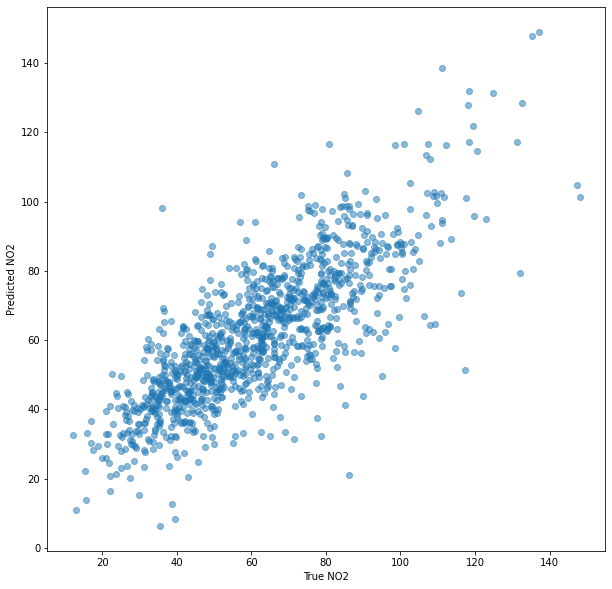
\includegraphics[width=\linewidth]{../catalogue/select-332a.png}
  \captionof{figure}{Scatterplot of the actual and predicted labels of a dataset. The visualisation shows that there is a linear relationship between the true and predicted labels.}
  \label{fig:r2}
\end{minipage}

Figure~\ref{fig:r2} shows a visualisation obtained from a notebook that trains a RNN to predict the levels of Nitrogen Dioxide ($NO_2$) in the next 24 hour window. The model is trained using time-series data consisting of historical readings of $NO_2$ and meteorological data such as temparate, humidity, wind speed, and such. The visualisation shows a scatterplot of the real and predicted values of $NO_2$ from the test set. The scatterplot shows a linear relationship between the ground truth and predictions indicating that the model was able to learn certain patterns in the training data. The spread of $y_{pred}$ at any given $y_{true}$ is wide. For example, at $y_{true} = 80$, the prediction can range anywhere between 30 and 120. This Indicates that the model was not able to fit the training data that well, and can be improved with fine-tuning.

% TODO more context on r2_score, it fits a linear regression model and checks the blah blah blah
Listing~\ref{lst:r2} presents the corresponding analytical test which was defined below Figure~\ref{fig:r2}. The author uses \texttt{r2\_score} metric from the scikit-learn library to quantify the performance of the model. The \texttt{r2\_score} method fits a linear regression model on the true and predicted labels and computed the Coefficient of Determination ($R^2$) based on the residuals of the linear regression model. The assertion checks that the $R^2$ score of the model is always higher than $0.6$. Since the best score possible is $1.0$, the specified threshold indicates that the author wants to ensure that $y_{pred}$ and $y_{true}$ are always linearly related to each other.

Similar to Figure~\ref{fig:svm}, the visualisation in Figure~\ref{fig:r2} allows ML practitioners to visually assess is the model is under or overfitting the training data. If the spread of $y_{pred}$ is wide, it indicates that the model is under-fitting. In contrast, if the spread is very close to the diagonal line, it indicates that the model is most likely overfitting. The visualisation can also be used to verify if there are any outliers in the predictions, for a given input. The assertion in Listing~\ref{lst:r2} however, does not capture such information. It can only check if the performance of the model is better than a specific threshold.

\subsection{Normalization}

% TODO check the notebook again for implementation of normalization

\begin{figure}
  \subcaptionbox{Histogram showing the distribution of a feature before and after scaling.\label{fig:scale}}{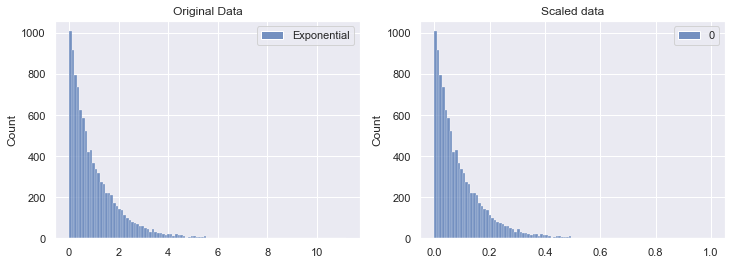
\includegraphics[width=0.45\linewidth]{../catalogue/select-65a.png}}
  \hfill
  \subcaptionbox{Histogram showing the distribution of a feature before and after normalisation.\label{fig:normal}}{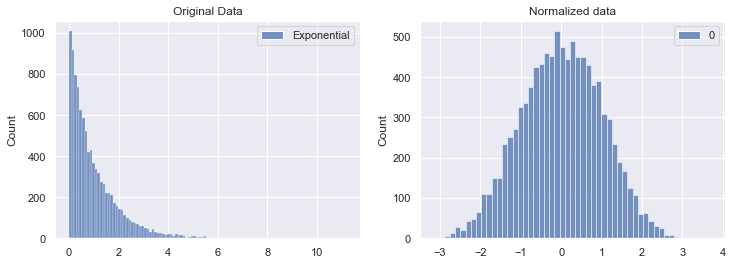
\includegraphics[width=0.45\linewidth]{../catalogue/select-65b.png}}
  \caption{Visualisation of data before and after various data pre-processing techniques.}
  \label{fig:data-pre-process}
\end{figure}

\begin{minipage}{0.45\textwidth}
  \begin{lstlisting}[language=Python]
assert scaled_data[scaled_data.argmax()] <= 1
assert scaled_data[scaled_data.argmix()] >= 0
  \end{lstlisting}
  \captionof{lstlisting}{Assertion to check that the mix and max of a feature fall within specified threshold derived from the visualisation presented in Figure~\ref{fig:scale}.}
  \label{lst:scale}
\end{minipage}
\hfill
\begin{minipage}{0.45\textwidth}
  \begin{lstlisting}[language=Python]
assert normalized_data[normalized_data.argmax()] < 10
assert normalized_data[normalized_data.argmin()] > -7
  \end{lstlisting}
  \captionof{lstlisting}{Similar premise as Listing~\ref{lst:scale}, however this assertion is based on Figure~\ref{fig:normal}.}
  \label{lst:normal}
\end{minipage}

Visualisations presented in Figure~\ref{fig:data-pre-process} were obtained from a notebook that presents a tutorial on scaling and normalization---two common data pre-processing techniques in ML. The visualisations show a comparison of the data before and after each pre-processing technique is applied to a feature from the data. The author scales the data using the \texttt{MinMaxScaler} from the scikit-learn library~\footnote{REFME}, between $[0, 1]$. The author performs a visual check, by comparing the distribution of the data before and after scaling, using a histogram (as shown in Figure~\ref{fig:scale}). Similarly, the author normalises the data using the \texttt{PowerTransformer} class from scikit-learn~footnote{REFME}, and performs a visual check as shown in Figure~\ref{fig:normal}.

Listing~\ref{lst:scale}~and~\ref{lst:normal} show the assertions that were defined below Figure~\ref{fig:scale}~and~\ref{fig:normal} respectively. Both assertions check that the min and max of the feature is within the expected bounds after applying the respective pre-processing technique. The assertion in Listing~\ref{lst:scale} is felt to be unneccessary since the min and max thresholds are set to the theoretical limits. The assertions in Listing~\ref{normal} are more relevant, however it is not clear why the author include such a wide margin in the thresholds.

\section{Discussion}\label{sec:discuss}

% NOTE comment on the over-whelming presence of magic thresholds in ML
% testing! where are authors getting these numbers from? link this to
% requirements engineering? 

% NOTE comment on the anti-patterns in testing that we observe in the 5 patterns presented

% NOTE link the qualitative and quantitative testing to the ML lifecycle: how some tests will let practitioner know when something changes

% NOTE comment on evolution? we have to look at the entire lifecycle of a visualisation: notebooks are run iteratively?

\subsection{New form of testing}
% NOTE some form of commentary on the fact that is form of qualitative and quantitative testing is happening but not that popular yet!

% NOTE so we need more tools to aid practitioners to encourage this form of testing and also help them translate qualitative properties into quantitative tests!

\subsection{From Implicit Expectations to Explicit Assertions}
% NOTE regeneration of the model does not change this observation at this point in time 

% NOTE discuss the pros and cons of having a qualitative assessment: they are dense with useful information; humans need visual patterns!

% NOTE then show that we also need qualitative assessment that can capture our expectations; this is important so that the model never violates that we understand from the visualisations

% NOTE now is the time to talk about how assertions act as documentation of the domain expertise and knowledge extracted from the visualisation from the original creator; this also scales as the system complexity and composition of the team/organisation evolves!

% NOTE what are the benefits using visualisations to assess the
% quality of ML systems? They are packed with a lot of
% information. And humans are cognitively tuned to identify patterns
% in visualisations.

Visualisations condense valuable information that is easy to understand for humans.

\subsection{Something about magic thresholds}\label{sec:magic-threshold}
% NOTE we observe that most analytical test translates to comparing a value against a threshold; this indicates the open challenges in ML testing; either we don't yet know how to translate analytical tests from visualisations or we cannot do this in the first place and we must use a hybrid approach?

% NOTE this is a better place to talk about the magic threshold phenomenon; link this to the magic number smell in software engineering, but in ML it is very prevalent and an alternative is not always clear

% NOTE and then motivate how we need more tools/techniques to aid practitioners to extract/translate all the info from visualisations into qualitative assertions!

\subsection{Humans need visual confirmation}\label{sec:visual}
% NOTE even though analytical tests are sufficient; humans still prefer visual confirmation

% NOTE when working with image dataset, we observe in our catalogue that practitioners prefers to also visually check the input image

% NOTE more detailed discussion on how a lot of information can be condensed into a single visualition and how humans are good at observing visual patterns

\section{Threats to Validity}\label{sec:threats}
% defend use of github as source for notebooks:
% - why did kaggle not work (refer to notes)
% - why did the existing replication packages not work?

% motivation for keeping the search on github broad:
% - not only does it pick up python assert statements, but also flags
% - notebooks that use other testing libraries or modules that provide a
% - testing interface. This is a good compromise between doing an
% - exhaustive search of all testing method names in the python
% - ecosystem and then doing a search for each of those patterns

% TODO don't mention quantity of random sample; then we need to explain/defend this choice
We used an iterative approach to determine the effectiveness of each
filter that was used. We applied each filter in the same order as
presented in Table~\ref{tab:filters}, starting with F1. We randomly
sampled 50 notebooks from the population of notebooks obtained after
applying the filter. We then conduct the qualitative assessment
presented in Section~\ref{REFME} and observe the number of related
visualisation and assertion pairs. In each new iteration, we
progressively add the other filters and include the filter if the
number of relevant visualisation and assertion pairs increases.
\section{Conclusion}\label{sec:conclude}

\bibliographystyle{IEEEtran}
\bibliography{bibliography}

\end{document}
\endinput

